\chapter{Design and Methods} \label{cha: designandmethods}
This Chapter first presents two hypothesis that guide the design and methods decisions. Second, the chosen \acs{ReID} and \acs{SR} models are presented, along with the losses and metrics used during training and validation. Finally, the different strategies for combining the two architectures are explored. The chapter is divided into three sections \ref{sec: Designreidmodule} \acs{ReID} Module,  \ref{sec:designSRmodule} \acs{SR} Module and \ref{combinednetworks} Combined XXXX, to maintain a clear and structured overview. 

\section{Hypotheses}\label{sec:hypotheses}
The chapters \ref{cha:problemanalysis} and \ref{cha: technicalanalysis} have outlined weaknesses and shortcomings in \acs{ReID} domain, as well as the potential of improvement when combined with \acs{SR}. Based on these insights, two hypotheses have been formulated to guide the subsequent analysis.

The experimental setups are built around the following hypotheses, and will be explained in the end of the chapter:
\begin{itemize}
    \item \textit{Hypothesis 1}: Training the \acs{ReID} module on augmented images will lead to more robust feature extraction.
    \item \textit{Hypothesis 2}: Running input through the \acs{SR} module, before it enters the \acs{ReID} module, will lead to better performance. 
\end{itemize}

As the project objective is to investigate how \acs{SR} can enhance the performance of \acs{ReID}, each component, presented in this chapter, was selected with the intent of establishing a fair and consistent foundation for comparison, rather than to achieve state-of-the-art results. Furthermore, both of the chosen model architectures have low parameter counts, for the purpose of solving the problem with design/architecture choices instead of relying on adding more parameters. 

\section{ReID Module} \label{sec: Designreidmodule}
This section introduces the chosen \acs{ReID} architecture, along with the training and test strategies, loss function and evaluation metrics. 

\subsection{OSNet} \label{sec:methodreid}
The \acf{OSNet} architecture presented in Section \ref{sec:omniscale} demonstrates strong performance across several person re-identification benchmarks \cite{OSNet}. The architecture is chosen as the \acs{ReID} module for this project based on its performance and the lightweight architecture, allowing for competitive accuracy that is not fueled by very many parameters. 
The details of the architecture are presented in this section, based on Figure \ref{fig:osnetpipeline}. 

\begin{figure} [H]
    \centering
    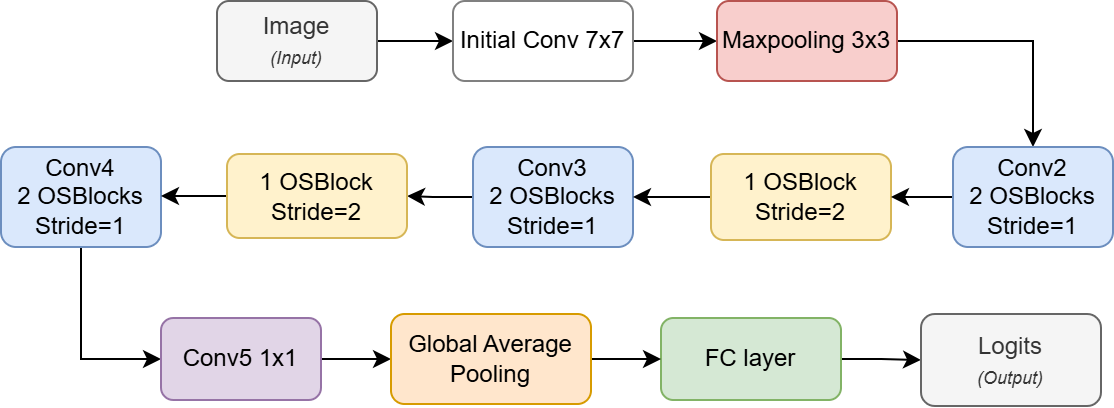
\includegraphics[width=1\linewidth]{osnetpipelinebud.png}
    \caption{An overview of the pipeline for the OSNet module.}
    \label{fig:osnetpipeline}
\end{figure}

\noindent As mentioned in Section \ref{sec:omniscale}, the model adaptively captures discriminative features for person \acs{ReID} across different spatial scales. This is achieved through \acf{OSBlock}, which are the fundamental building units of \acs{OSNet}. The full pipeline of \acs{OSNet} is presented in Figure \ref{fig:osnetpipeline}, while the internal process of a single \acs{OSBlock} is presented in Figure \ref{fig:osblockpipeline}. 

\begin{figure} [H]
    \centering
    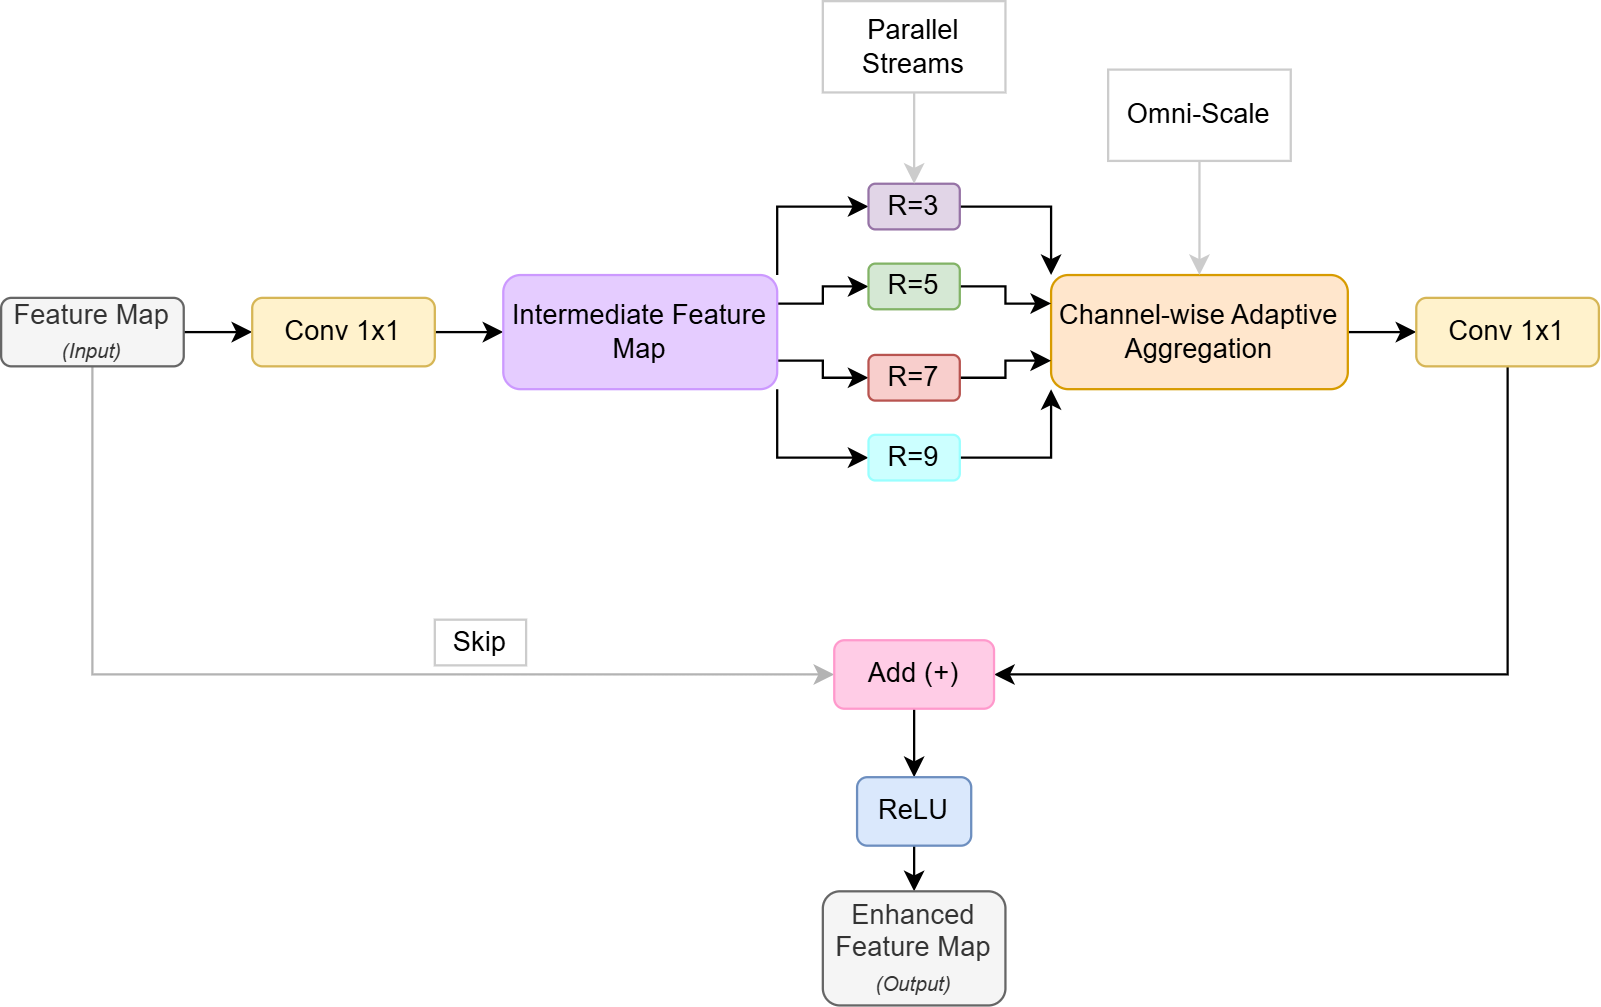
\includegraphics[width=1\linewidth]{osblockpipeline.png}
    \caption{An overview of the process inside the \acs{OSBlock}s.}
    \label{fig:osblockpipeline}
\end{figure}

\noindent The first \acs{OSBlock} receives a feature map created by an initial convolution and maxpooling, with the following \acs{OSBlock}s taking the feature map from the previous layer. In these blocks, the feature map is processed by a \textit{1x1} convolution, which reduces the channel dimensions. Subsequently, four parallel streams apply convolutions with kernel sizes \textit{3x3}, \textit{5x5}, \textit{7x7}, and \textit{9x9}, corresponding to increasing receptive fields, to capture features at different scales, which defines the omni-scale capability. Each branch uses depthwise separable convolutions, also called lite \textit{3x3}, to improve efficiency. The output from all four streams is then aggregated with channel-wise adaptive aggregation to dynamically weigh each scale based on the input. The aggregation is implemented with a lightweight gating mechanism, that learns to weigh each scale adaptively. This fusion is what makes the model omni-scale. After the fusion, a \textit{1x1} convolution restores the original channels. The final result is added to the input of the block by a skip connection and passed through a ReLU activation function. Each stage contains two \acs{OSBlock}s with \texttt{stride=1}, before an \acs{OSBlock} with \texttt{stride=2} downsamples the feature map. 
\\\\
This process is repeated until the fourth convolution stage, which is followed by a \textit{1x1} convolution, to fuse information across all channels. Global average pooling is used to collapse the spatial dimensions into one value per channel resulting in a feature vector, which is passed through a fully connected layer to produce the final embedding that is used for person re-identification.  

\subsubsection{Model Configuration}
\acs{OSNet} comes in 4 size configurations, varying in depth and width \cite{OSNet}. In this project, the full-size \acs{OSNet}\_x1.0 variant is used with 2.2 million parameters. As shown in Table \ref{tab:osnet-config} the model consists of three stages of \acs{OSBlock}s using channel configurations of [64, 256, 384, 512]. The model was initialized with random weights (\texttt{pretrained=False}) rather than using pretrained, ensuring that the model learns features specially relevant to the combined datasets.
\begin{table}[H]
    \centering
    \begin{tabular}{|c|c|}\hline
        \cellcolor[HTML]{D8E9F7} \textbf{Parameter} & \cellcolor[HTML]{D8E9F7} \textbf{Value} \\\hline
        No. Classes (\texttt{num\_classes}) & \texttt{num\_classes} \\\hline
        Block types (\texttt{blocks})             & [\texttt{OSBlock}, \texttt{OSBlock}, \texttt{OSBlock}] \\\hline
        Layers per stage (\texttt{layers})        & [2, 2, 2] \\\hline
        Channels per stage (\texttt{channels})    & [64, 256, 384, 512] \\\hline
    \end{tabular}
        \caption{OSNet\_x1\_0 Configuration.}
    \label{tab:osnet-config}
\end{table}

\subsection{Loss Function}
The choice of a loss function is fundamental to the optimization process and to shaping the representations learned by the model \cite{lossfunction}. In person \acs{ReID} tasks, the loss function must encourage the learning of discriminative features that can separate identities while remaining efficient during training. In addition, an open-set problem, as \acs{ReID} is, requires the model to generalize effectively to identities not seen during training. This section introduces the loss function used for \acs{OSNet} and explains how it supports effective feature learning for identity classification.

\subsubsection*{Multiclass Cross-Entropy Loss}
Multiclass cross-entropy loss, also known as softmax loss, is commonly used for classification tasks where each input has one correct class \cite{softmax}. It works by applying a softmax function to the model's output logits to produce a probability distribution for each class, and then calculating the negative log-likelihood of the true class. The following formula shows the softmax loss written directly in terms of logits, as presented in \cite{softmax}:

\[
\mathcal{L}_i = - f_{y_i} + \log \sum_{j} e^{f_j}
\]

\begin{description}
    \item[$\mathcal{L}_i$]: Softmax loss for the $i$-th sample.
    \item[$f_{y_i}$]: Logit corresponding to the true class.
    \item[$y_i$]: Ground-truth class index for sample $i$.
    \item[$f_j$]: Logit for class $j$.
    \item[$\sum_j e^{f_j}$]: Normalization term over all classes.
\end{description}

\noindent This encourages the model to assign a high probability score to the correct class, while penalizing confident but incorrect predictions. The output probabilities can be interpreted as the model's confidence in each class. However, these probabilities are influenced by the scale of the model's logits, which is affected by the regularization strength used in training. Stronger regularization punishes large parameter values, which can reduce the scale of the logits and result in softer softmax outputs. In contrast, lower regularization may allow for larger softmax outputs. Label smoothing is a regularization technique commonly used in combination with softmax loss, as it prevents the model from becoming overconfident in its predictions, by softening the target labels instead of using one-hot encoded labels \cite{labelsmoothing}. This is particularly beneficial for person \acs{ReID}, as it addresses the challenge of limited training samples per identity. By preventing extreme confidence on training identities, label smoothing encourages the model to learn more robust features that generalize better to unseen test identities, a critical requirement for the open-set nature of person \acs{ReID}.

\subsection{Evaluation Metrics}
The evaluation metrics help measure how well the models perform on a given task \cite{evaluationmetrics}. Therefore, selecting the appropriate metrics is essential to ensure that the evaluation reflects the objective of the task. In the context of person \acs{ReID}, the evaluation must capture the model's ability to correctly identify individuals, as well as the quality of the ranking of retrieved matches. This section introduces the evaluation metrics used for the person \acs{ReID} module.

\subsubsection*{Rank}
Rank-\textit{k} metrics are widely used in \acs{ReID} to measure how good the system is at getting a correct identity match within a certain range. Rank is based on a concept called the Cumulative Matching Characteristic, which describes the probability that the first correct match appears within the top \textit{k} results of all queries evaluated.
\\\\
For example, a Rank metric with \texttt{k = 1} would answer the question "For how many queries were the top match the correct identity?" while a Rank with \texttt{k = 5} would answer "For how many queries did the correct identity appear in the top 5 matches?". This is the same with different valued \textit{k's}, just with more or less of the matches for the queries accounted for. Because it is a Cumulative Metric, it will count a query as a success if the correct match is within the top \textit{k} positions. In other words, once a query has its first correct match at rank \textit{r}, it is counted as a success for all Rank-\textit{k} metrics where \(k \ge r\). This is done on multiple queries where an average is then taken of the successes for each Rank-\textit{k} \cite{rankmetricEvidently}. 
\\\\
In short, Rank-\textit{k} describes the models ability to find a correct match in top-\textit{k}, making it ideal as evaluation metric for this project.

\subsubsection*{\acs{mAP}}
\acf{mAP} is a commonly used metric to examine the performance of both object detection and information retrieval systems, such as \acs{ReID}. \acs{mAP} can differ depending on what it is being used for, but in a \acs{ReID} context, it works by measuring how good the system is at retrieving the correct identities across the entire ranked gallery list, which also makes it ideal to work alongside the Rank-\textit{k} metric, as it estimates all true matches, and not just a given \textit{k} range. As the name implies, \acs{mAP} is found by calculating the mean of the overall Average Precisions of all valid queries. In \acs{ReID}, Average Precision is computed from the ranked gallery list by measuring precision at every correct match starting from the highest similarity score to the lowest. An average of these precisions is then taken to get the Average Precision of that query. Meanwhile, \acs{mAP} is the mean of those Average Precisions across all the valid queries. This means it both accounts for how good the system is at finding matches, but also how good it ranks them \cite{mAPlightly}. Because \acs{mAP} evaluates the model’s ability to retrieve all relevant matches, it is selected as the primary metric for model selection.

\subsection{Training Strategy}
The \acs{ReID} module were trained on a combination of Market-1501 \cite{CVATM1501}, MSMT17 \cite{wei2018person} and CUHK03 \cite{KaggleCUHK03}, providing 2,117 unique identities across diverse surveillance conditions. This multi dataset approach was chosen to ensure that the model learns generalizable features rather than dataset-specific patterns. Each dataset contributes distinct characteristics: Market-1501 provides realistic detector noise, CUHK03 offers both manual and automatic detected annotations, and MSMT17 contributes with 15 cameras across indoor and outdoor scenes, captured at different times of day.

\subsection{Testing Strategy}\label{Reidteststrategy}
Evaluation follows a two stage approach, In distribution testing on MSMT17, Market-1501, and CUHK03 establishes a baseline performance on known datasets. The primary focus is \acs{OOD} testing using DukeMTMC-\acs{ReID} serves as a same domain \acs{OOD} test with outdoor university surveillance similar to the training datasets, but with a new demographic and environment. \acs{iLIDS-VID} provides a cross domain test with indoor airport footage, evaluating whether the model learned truly discriminative features or over fitted to outdoor characteristics. Beyond dataset shifts, controlled degradations are applied to DukeMTMC-ReID: scale reduction (0.75, 0.5, 0.25) and JPEG compression (quality 50, 25, 15). These simulate realistic surveillance challenges where persons appear at varying distances or footage is compressed for storage, directly testing the projects core hypothesis \acs{SR} can reduce resolution degradation effects on \acs{ReID} performance. 

\section{Dataaugmentation} \label{sec: dataaugmentation}
To test if the first hypothesis is true both a baseline and robust version of the \acs{ReID} Module is created, so a fair comparison can be made. This is done through different augmentation pipelines. As the goal is to improve model performance in terms of generalization across different image scales and resolution, for robustness in real life scenarios. The different types of augmentation and their purpose is included in Table \ref{tab:augmentationtypes}.
\begin{table}[H]
    \centering
    \begin{tabular}{|>{\centering\arraybackslash}p{0.18\linewidth}|>{\centering\arraybackslash}p{0.78\linewidth}|}\hline
         \cellcolor[HTML]{D8E9F7} \textbf{Augmentation}&  \cellcolor[HTML]{D8E9F7} \textbf{Purpose}\\\hline
         Horizontal flipping&  Increase dataset size.\\\hline
 Gaussian blur&Improve robustness to low-quality or blurred images.\\\hline
 Gaussian noise&Enhance generalization to imperfect or noisy images.\\\hline
 Brightness change&Increase resilience to varying lighting conditions.\\\hline
 Resizing&Introduces scale variation by randomly reducing the image size with a scale between 0.5 and 1 and then black padding back to the target dimensions. Resizing is performed with bilinear interpolation.\\\hline
 Padding& Secure that tensor sizes is the same in order to be stacked.\\\hline
 JPEG compression& Improve robustness to compression noise, simulating compression from surveillance footage.\\ \hline
    \end{tabular}
    \caption{The different augmentations implemented.}
    \label{tab:augmentationtypes}
\end{table}
\noindent These data augmentations were used in two different transformation pipelines: One with light augmentations for baseline version, one with strong augmentations for the robust version, see Table \ref{tab:three_subtables}.
\begin{table}[H]
\centering
\begin{subtable}[T]{0.32\linewidth}
\centering
\begin{tabular}{|>{\centering\arraybackslash}p{0.9\linewidth}|}\hline
\cellcolor[HTML]{D8E9F7} \textbf{Light Training Augmentation}\\\hline
\begin{itemize}[leftmargin=*, topsep=0pt, itemsep=0pt]
    \item Horizontal flipping
    \item Padding, if too small
    \item Resizing, if too big
    \vspace{6.1em}
\end{itemize}
\\ \hline\end{tabular}
\caption{Augmentations used for baseline version of OSNet.}
\end{subtable}
\begin{subtable}[T]{0.32\linewidth}
\centering
\begin{tabular}{|>{\centering\arraybackslash}p{0.9\linewidth}|}\hline
\cellcolor[HTML]{D8E9F7} \textbf{Strong Training Augmentation}\\\hline
\begin{itemize}[leftmargin=*, topsep=0pt, itemsep=0pt]
    \item Gaussian noise
    \item Gaussian Blur
    \item Brightness change
    \item Resizing
    \item JPEG compression*
    \item Horizontal flipping
    \vspace{1em}
\end{itemize}
\\ \hline\end{tabular}
\caption{Augmentation used for robust version of OSNet.}
\end{subtable}
\caption{The two different augmentations pipelines.}
\label{tab:three_subtables}
\end{table}

\section{SR Module}\label{sec:designSRmodule}
This section presents the chosen \acs{SR} architecture, as well as the training strategy using the two \acs{SR} datasets presented in Section \ref{sec: superresdata}. Based on the technical analysis of the perception-distortion trade of in the SR domain presented in \ref{subsec:perception-distortion-tradeoff}, a low distortion model is considered more suitable for integration with \acs{ReID}, as it reduces the risk for introduction of SR artifacts.

\subsection{EDSR}
\acf{EDSR} is a \acs{ResNet} based architecture for single image \acs{SR}, designed with an emphasis on high reconstruction quality and stable training. As mentioned in Section \ref{sec: edsr relatedworks}, \acs{EDSR} showed strong performance when optimizing for low distortion, making it a promising candidate as a pre-processing unit for the task of \acs{ReID}.
\\\\
The architecture consists of a convolutional layer, a deep stack of residual blocks and an upsampling module that produces the super-resolution output for the given scale factor. The overall \acs{EDSR} pipeline can be seen in Figure \ref{fig:edsrpipeline}, the internal flow of each resblock is illustrated in Figure \ref{fig:resblockpipeline}, and the process inside the final upsample block can be seen in Figure \ref{fig:upsampleblockpipeline}. 
\begin{figure} [H]
    \centering
    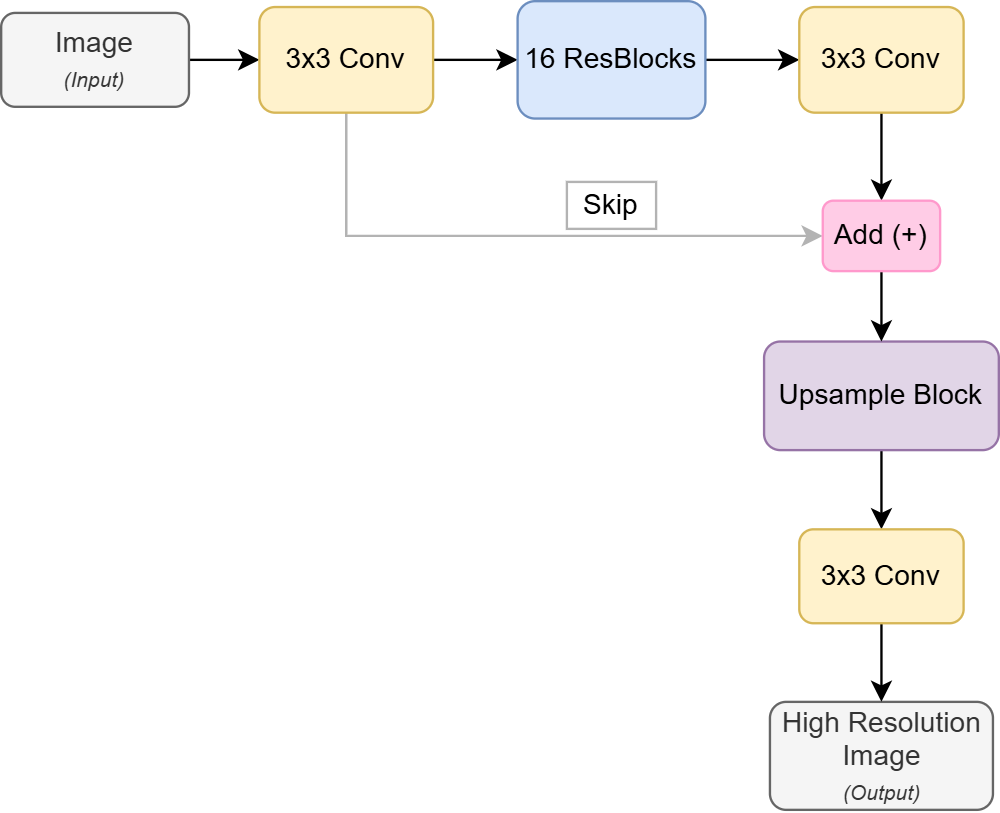
\includegraphics[width=0.75\linewidth]{edsrpipeline.png}
    \caption{An overview of the \acs{EDSR} pipeline.}
    \label{fig:edsrpipeline}
\end{figure}

\noindent Similar to the \acs{ResNet} architecture, \ac{EDSR} has multiple skip connections enabling the training of deeper networks without suffering from vanishing gradient. These skip connections also improve feature refinement by allowing the network to focus on learning the residual improvements to the input, rather than storing the entire input in memory. In total \ac{EDSR} has two types skip-connections, one in each of the resblocks, see Figure \ref{fig:resblockpipeline} and one, from the first convolutional layer adding just before the upsampling block, see Figure \ref{fig:edsrpipeline}.

\begin{figure} [H]
    \centering
    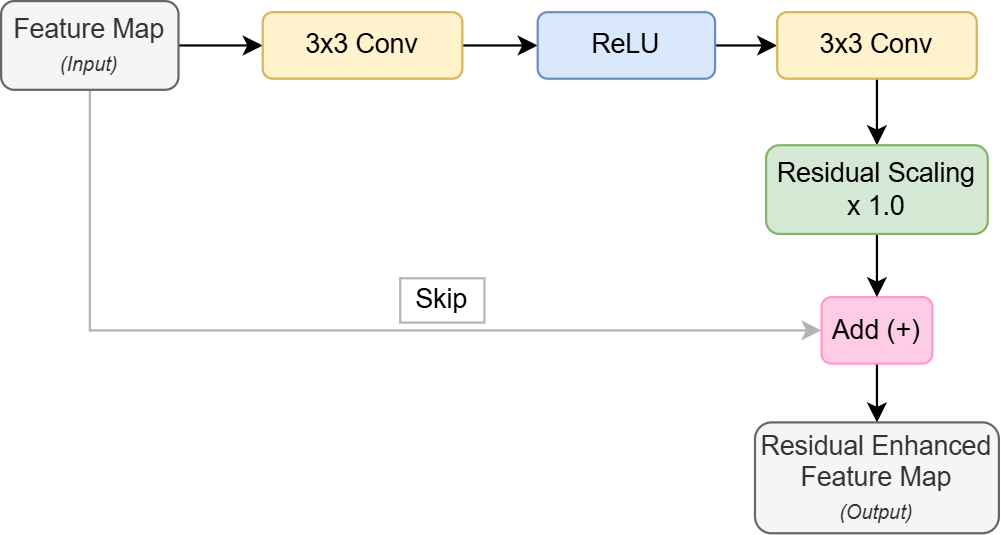
\includegraphics[width=0.75\linewidth]{resblockpipeline.png}
    \caption{An overview of the internal process of the resblocks.}
    \label{fig:resblockpipeline}
\end{figure}

\noindent As \acs{EDSR} is a deep and wide model, residual scaling is commonly employed to stabilize training by multiplying the output of each residual block with a small factor before adding it to the skip connection. However, this does not apply to the baseline model used in this work, as it is the smallest configuration and employs a residual scaling factor of 1, which effectively corresponds to no residual scaling.


\begin{figure} [H]
    \centering
    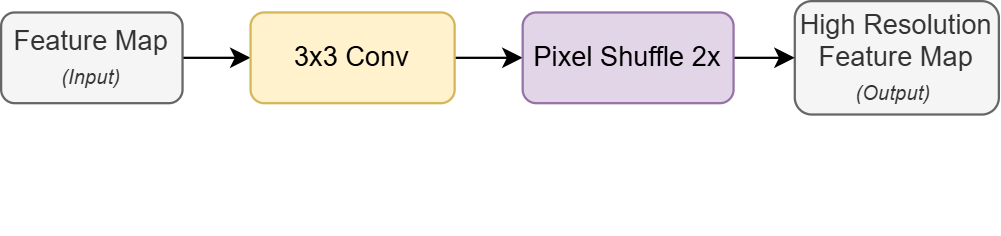
\includegraphics[width=0.75\linewidth]{upsampleblockpipeline.png}
    \caption{An overview of the internal process of the upsample block.}
    \label{fig:upsampleblockpipeline}
\end{figure}

\noindent As shown in Figure \ref{fig:edsrpipeline}, the upsampling stage is implemented by learnable upsampling modules placed at the end of the network, so that most of the computation is performed in the low-resolution space, effectively meaning only the final layers project the feature maps to high resolution. In Figure \ref{fig:upsampleblockpipeline}, the pipeline of the upsampling module is visualized. It uses a sub-pixel convolution approach called \texttt{PixelShuffle}, where a convolutional layer first expands the feature maps by a factor of scale\textsuperscript{2} and the \texttt{PixelShuffle} operation then rearranges these features into the spatially upscaled output \cite{shi2016subpixel_arxiv}. This approach performs upsampling in a learnable manner rather than using fixed interpolation methods.

\subsection{Loss Function}
For the training of the \acs{SR} module, mean absolute error (MAE), also called L1 loss, was used as the training objective. MAE was chosen over mean squared error, MSE or L2 loss, because it produces sharper reconstructions and is less sensitive to outliers in the training data.\footnote{Kilde skal indsættes her for påstanden om L1 loss robusthed over for outliers.} 

\subsection{Evaluation Metric}
PSNR does ditten og datten

\subsection{Training and Validation Strategy}
A two-stage training strategy was employed. First, the model was pretrained on the RELLISUR dataset, followed by finetuning on \acs{DIV2K}. This approach was chosen instead of mixing the datasets directly due to their fundamentally different degradation characteristics. RELLISUR consists of real low-light and low-resolution image pairs captured under natural imaging conditions, where degradations arise from the physical image acquisition process rather than synthetic downsampling.

By pretraining on RELLISUR, the model is exposed to realistic degradation patterns, allowing it to learn robust representations for handling real-world low-light super-resolution. Subsequent finetuning on \acs{DIV2K}, which contains high-quality images with synthetically generated low-resolution counterparts, refines these representations under controlled degradation settings. This finetuning stage improves reconstruction stability and generalization while retaining the realism learned during pretraining.

\subsection{Data Augmentation}
As the XXXX is to make \acs{SR} to remove
\begin{table}[T]{0.32\linewidth}
\centering
\begin{tabular}{|>{\centering\arraybackslash}p{0.9\linewidth}|}\hline
\cellcolor[HTML]{D8E9F7} \textbf{EDSR Training Augmentation}\\\hline
\begin{itemize}[leftmargin=*, topsep=0pt, itemsep=0pt]
    \item Gaussian noise
    \item Gaussian Blur
    \item Brightness change
    \item Resizing
    \item JPEG compression*
    \item Horizontal flipping
    \vspace{1em}
\end{itemize}
\\ \hline\end{tabular}
\caption{Augmentation used for \acs{SR} module.}
\label{edsraugmentation}
\end{table}
*By mistake, JPEG compression was not applied to the EDSR pipeline. The consequences of this mistake are discussed in Section XXX.

\section{Combining Architectures}\label{combinednetworks}

\subsection{Sequential}

\subsection{Joint end-to-end integration}

\section{Summary}
During the chapters different XXXX
The finding during this chapter leads to definition of four implementations, what is explored in order to find a solution to the two hypothesis.

\begin{itemize}
    \item Baseline model of \acs{OSNet} trained using the light augmentations.
    \item Robust model of \acs{OSNet} trained using the strong augmentations.
    \item Baseline model of \acs{OSNet} in sequential combination with \acs{EDSR}.
    \item Baseline model of \acs{OSNet} trained jointly end-to-end with \acs{EDSR}.
\end{itemize}


The integration can be executed in a multitude of ways. In this project, only some of these implementation will be explored. 
 
Et eller andet .... dette chapter vil investigate how to do se, and then experiments will be set...

in order to test, what improves the in- and out-of-distribution performance of the \acs{ReID} model, which are defined in Section \ref{Reidteststrategy}. 

This will be explored at two levels of integration:
    \begin{itemize}
        \item \textit{Integration 1}: Sequential integration, where input is first processed through the \acs{SR} module, before it enters the \acs{ReID} module.
        \item \textit{Integration 2}: End-to-end integration such that \acs{ReID} losses can back-propagate into the \acs{SR} module.
    \end{itemize}




%For the evaluation of the models and systems in our project, \ac{mAP} and Rank was calculated similarly as explained above with some minor additional steps, like filtering out images that has multiple images 

%The \ac{mAP} metric is made up of multiple other sub metrics, such as \ac{IoU}, Recall, and Precision, that are important to understand to grasp how the \ac{mAP} works, and how it is correctly calculated. 

%Average Precision is computed by finding the area under the precision-recall curve, where precision is the proportion of true positive and false positive matches, while recall is the proportion of true positives out of all possible positive matches

% Firstly, a filter was applied to only keep the good matches in the gallery, and After the trained OSNet model extracts the features and calculates the distance/similarity of the query and gallery with \texttt{torch.cdist}, all of the gallery images are sorted by the given similarity with the query. Before being  Afterwards the Average Precision is found based on the matches in each query, and then \ac{mAP}

%Because its a Cumulative Metric, it will count a query as a success if there is a match within the certain k-range of that query. For example, if a query had its first correct identity match at Rank-3, a Rank-10 metric would count that query as a success, as that specific metric asks "Is there a correct match within 10 matches?" for each query.

%,  and after the trained OSNet model extracts the features and calculates the distance/similarity of the query and gallery with \texttt{torch.cdist}, all of the gallery images are sorted by the given similarity with the query. Before being 


% reid_test.py has mAP = sum(aps) / valid queries, where aps is a list of "ap", and ap = sum(precisions) / len(precisions) that is appended to aps. And precisions is a list of "hits/(pos+1)" in a for loop that has "for pos in pos_idx". And pos_idx is "pos_idx = good.nonzero(as_tuple=False).view(-1)" which is described as indices for True in good. While good is "good = matches[i][order]

